%
% abb.tex -- Abbildungsgleichung
%
% (c) 2018 Prof Dr Andreas Müller, Hochschule Rapperswil
%
\documentclass[tikz,12pt]{standalone}
\usepackage{times}
\usepackage{amsmath}
\usepackage{txfonts}
\usepackage[utf8]{inputenc}
\usepackage{graphics}
\usepackage{color}
\usepackage{pifont}
\usetikzlibrary{arrows,intersections,math,calc}
\begin{document}

\def\punkt#1{
        \fill[color=white] #1 circle[radius=0.08];
        \draw #1 circle[radius=0.08];
}

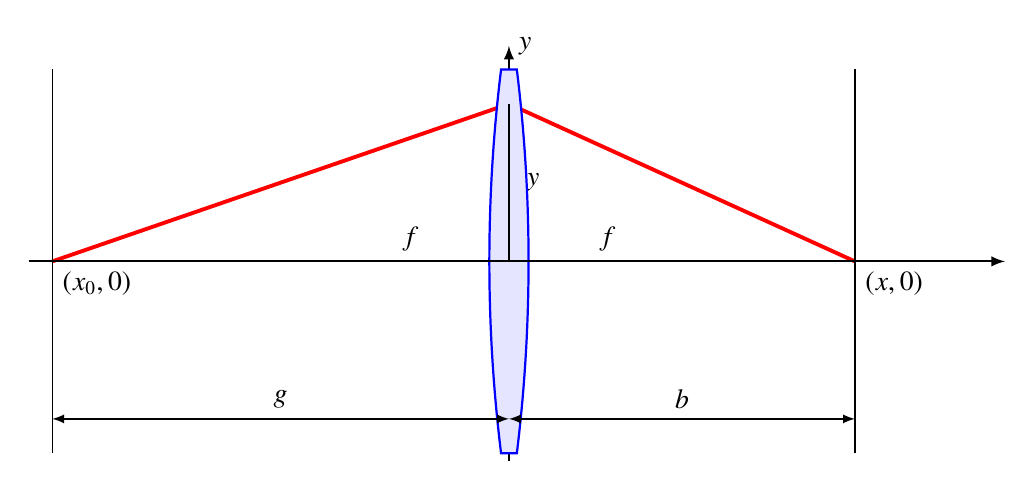
\begin{tikzpicture}[>=latex,thick]

\def\w{6}
\def\a{7}
\def\R{20}
\def\d{0.1}
\def\f{2.5}

\def\g{5.8}
\pgfmathparse{1/(1/\f-1/\g)}
\xdef\b{\pgfmathresult}

\pgfmathparse{\R*sin(\a)}
\xdef\h{\pgfmathresult}

\draw[->,line width=0.7pt] (0,{-\h-0.1})--(0,{\h+0.3})
	coordinate[label={right:$y$}];

\draw[line width=1.4pt,color=red] (-\g,0)--(0,2)--(\b,0);

\fill[color=blue!10]
	({-\d},{\h}) arc (180-\a:180+\a:\R)
	--
	({\d},{-\h}) arc (-\a:+\a:\R)
	--cycle;

\draw[line width=0.5pt] (0,0)--(0,2);
\node at (0.1,1) [right] {$y$};
\punkt{(0,2)}

\draw[color=blue]
	({-\d},{\h}) arc (180-\a:180+\a:\R)
	--
	({\d},{-\h}) arc (-\a:+\a:\R)
	--cycle;

\draw[->,line width=0.7pt] ({-\w-0.1},0)--({\w+0.3},0);

\draw[line width=0.5pt] ({-\g},{\h})--({-\g},{-\h});
\draw[line width=0.5pt] ({\b},{\h})--({\b},{-\h});

\draw[<->,line width=0.5pt] ({-\g},-2)--(0,-2);
\node at ({-\g/2},-2) [above] {$g$};

\draw[<->,line width=0.5pt] ({\b},-2)--(0,-2);
\node at ({\b/2},-2) [above] {$b$};

\punkt{(\f,0)}
\punkt{(-\f,0)}

\node at ({-\f/2},0) [above] {$f$};
\node at ({\f/2},0) [above] {$f$};

\punkt{(-\g,0)}
\punkt{(\b,0)}

\node at ({-\g},0) [below right] {$(x_0,0)$};
\node at ({\b},0) [below right] {$(x,0)$};

\end{tikzpicture}

\end{document}

